%\documentclass[twocolumn]{article}
\documentclass{article}

%\usepackage{arxiv}



\usepackage[utf8]{inputenc} % allow utf-8 input
\usepackage[T1]{fontenc}    % use 8-bit T1 fonts
\usepackage{hyperref}       % hyperlinks
\usepackage{url}            % simple URL typesetting
\usepackage{booktabs}       % professional-quality tables
\usepackage{amsfonts}       % blackboard math symbols
%\usepackage{nicefrac}       % compact symbols for 1/2, etc.
%\usepackage{microtype}      % microtypography
\usepackage{lipsum}		% Can be removed after putting your text content
\usepackage{graphicx}
%\usepackage{natbib}
\usepackage{doi}
\usepackage{amsmath}

%\usepackage{biblatex}

\usepackage{grffile}
\usepackage{authblk}

\usepackage[switch,columnwise]{lineno}
\linenumbers
\usepackage{fixmetodonotes}
\usepackage{multirow} % Needed for merging cells vertically
\usepackage{makecell} % For multi-line cells
\usepackage{booktabs} % For nicer table lines
\usepackage{adjustbox} % For table adjustments

% Import bibliography
%\bibliography{anoruti_refs.bib}
%\addbibresource{anoruti_refs.bib}


%opening
\title{Modeling the dynamics of bacterial colonisation in a murine model of Urinary Tract Infections}
\author[1]{Carlos Olivares}
\author[1]{Charles Burdet}
\author[1]{Ariane Amoura}
\author[1]{Imane El Meouche}
\author[1,2]{Emmanuelle Comets}

\affil[1]{Universit\'e Paris Cit\'e and Universit\'e Sorbonne Paris Nord, Inserm, IAME, F-75018 Paris, France}
\affil[2]{Univ Rennes, Inserm, EHESP, Irset - UMRS 1085, 35000 Rennes, France}
%\institute[shortinst]{\inst{1} \textit{Universit\'e Paris Cit\'e and Universit\'e Sorbonne Paris Nord, Inserm, IAME, F-75018 Paris, France} \samelineand \inst{2} \textit{Univ Rennes, Inserm, EHESP, Irset - UMRS 1085, 35000 Rennes, France}}


\begin{document}

\maketitle

\begin{abstract}
	
\TODO{Change Abstract}
Ariane's paper summary:

Urinary tract infection (UTI), mainly caused by Escherichia coli, are frequent and have a recurrent nature even
after antibiotic treatment. Potential bacterial escape mechanisms include growth defects, but probing bacterial division in vivo and establishing its relation to the antibiotic response remain challenging. Using a synthetic reporter of cell division, we follow the temporal dynamics of cell division for different E. coli clinical
strains in a UTI mouse model with and without antibiotics. We show that more bacteria are actively dividing in the kidneys and urine compared with the bladder. Bacteria that survive antibiotic treatment are consistently non-dividing in three sites of infection. 
Additionally, we demonstrate how both the strain in vitro persistence profile and the microenvironment impact infection and treatment dynamics. Understanding the relative
contribution of the host environment, growth heterogeneity, non-dividing bacteria, and antibiotic persistence is crucial to improve therapies for recurrent infections.
\end{abstract}

\section{Introduction}



\begin{itemize}
	\item Importance, motivation Why?
	\item What is know about it?
	\item What is the purpose of this work?
	\item Migration dynamics depends on the bacteria strain.
	\item Urinary tract infections (UTI) are the second most common infection worldwide with high recurrence rates, with E. coli the most prevalent cause of infection \cite{rosen2007detection}.
	\item Understanding the survival mechanisms and prevalence of these pathogens plays an important role in avoiding resistant bacteria's appearance and proliferation and tolerance.
	\item How to explain that non-dividing bacteria are the ones that survives?
\end{itemize}

\section{Methods}






\subsection{Data Description}
\TODO{Change or remove sampling figure, maybe better to add numbers with the symbols or just text description.}
\begin{figure}
	\centering
	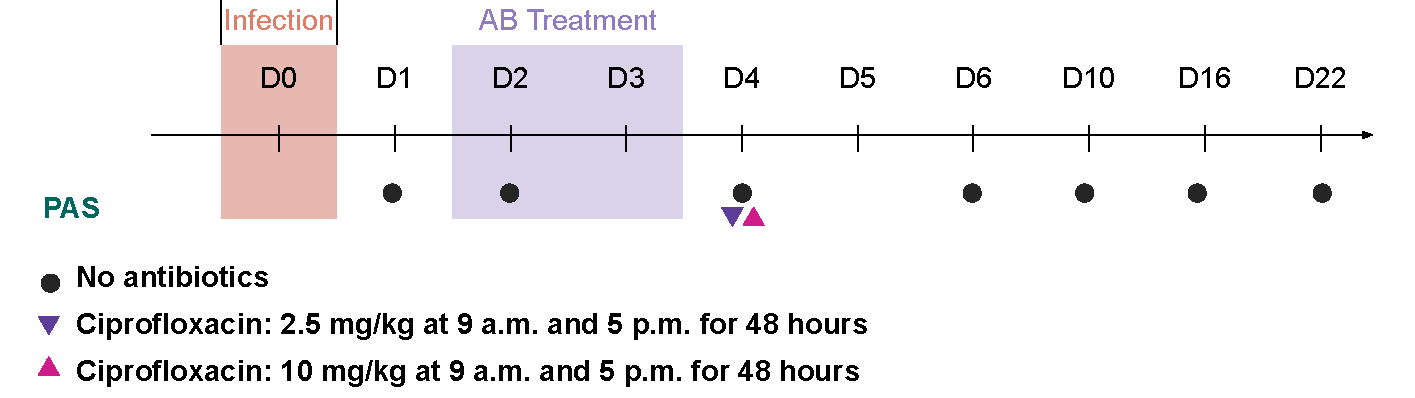
\includegraphics[width=0.8\linewidth]{images/draw_Anoruti_flowchart_PAS.pdf}
	\caption{Data description. }
	%		\label{fig:ModelOneline}
\end{figure}

%draw_Anoruti_flowchart_PAS

A total of \TODO{(Add the correct number when finish if all strains with all ATB or not)} 8-week-old healthy female CBA/J mice were intravesically infected, at day 0, with $10^8$ colony forming units (CFU) of PAS strain\cite{kotula2014programmable} and divided in three groups\cite{amoura2024variability}(76 mice without antibiotic, 17 with 2.5mg/kg and 7 with 10 mg/kg of ciprofloxacin during 2 days of treatment two times a day).




The CFU counts in each organ were determined by scaling the density of CFU/g measured in kidney and bladder by the organ weight after sacrifice. For urine, a scaling factor of 1ml was assumed. Mice without antibiotic treatment were sacrificed on days 1, 2, 4, 6, 10, 16 and 22. Mice with antibiotic treatment were only sacrificed on day 4.


\begin{itemize}
	\item \TODO{Add table with mice organ distribution CFU counts? or write directly med [min;max]}
	\item \TODO{LacZ too? Let's see that later}
\end{itemize}


\subsubsection{Ethics Statement} 
\TODO{The study was conducted in accordance with the ethical standards of ... and received approval from the ... }

\subsection{Statistical model}

Nonlinear mixed effects modeling approach was used to analyze the different markers over time. A nonlinear mixed effects model for multiple responses is defined as follows. Let $y_i$ denote the vector of observations for all responses and  the vector $y_{i,k}$ of observations for the $k$th response (e.g. k=1 corresponds to CFU in kidney, k=2 to CFU in bladder, etc) for the individual $i$. Let $f$ denote the global structural model characterizing all responses, based on a system of ordinary differential equations, similar for all individuals.
Then one can define $ y_{i,k} = f_{k}(\theta_i, \xi_{i,k} ) + \epsilon_{i,k} $ where $f_{k}$ is the component of the global model $f$ describing the $k$th response, $\theta_i$ is the vector of individual parameters, $\xi_{i,k}$ is the vector of the $n_{i,k}$ sampling times and $\epsilon_{i,k}$ is the vector of residual errors for the  response in individual $i$. Each individual parameter $\theta_i$ can be decomposed as a fixed effect $\mu$, which represents the mean value of the parameter in the population, and a random effect $b_i \sim \mathcal{N}(0, \Omega)$ where $\Omega$ accounts for the inter-individual variability. Assuming an exponential random effect model, the individual parameters are modeled as : $\theta_i = \mu \exp(b)$.
Lastly we assumed that $\epsilon_{i,k} \sim \mathcal{N} (0, \Sigma_{i,k})$ where $\Sigma_{i,k}$ is a $ n_{i,k} \times n_{i,k}$-diagonal matrix with $k$th elements equal to $(\theta_{inter,k} + \sigma_{slope,k}\times f_{k}(\theta_i, \xi_{i,k}))^2$ with $\sigma_{inter, k}$ being the paremeter for the additive part and $\sigma_{slope,k}$ the parameter for the proportional part of the variance error model. Constant ($\sigma_{inter, k} \neq 0$, $\sigma_{slope, k} = 0$), proportional ($\sigma_{inter, k} = 0$, $\sigma_{inter, k} \neq 0$, ) or combined ($\sigma_{inter, k} \neq 0$, $\sigma_{slope, k} \neq 0$ ) variance error models were tested for each response $k$.





\subsection{Modeling Strategy}
\TODO{Define order strain or antibiotic effect first? I think is better strain, because antibiotic has less data perhaps?}
\TODO{Make a better figure \ref{fig:ModelingStrategy} and include the strains}
\begin{figure}
	\centering
	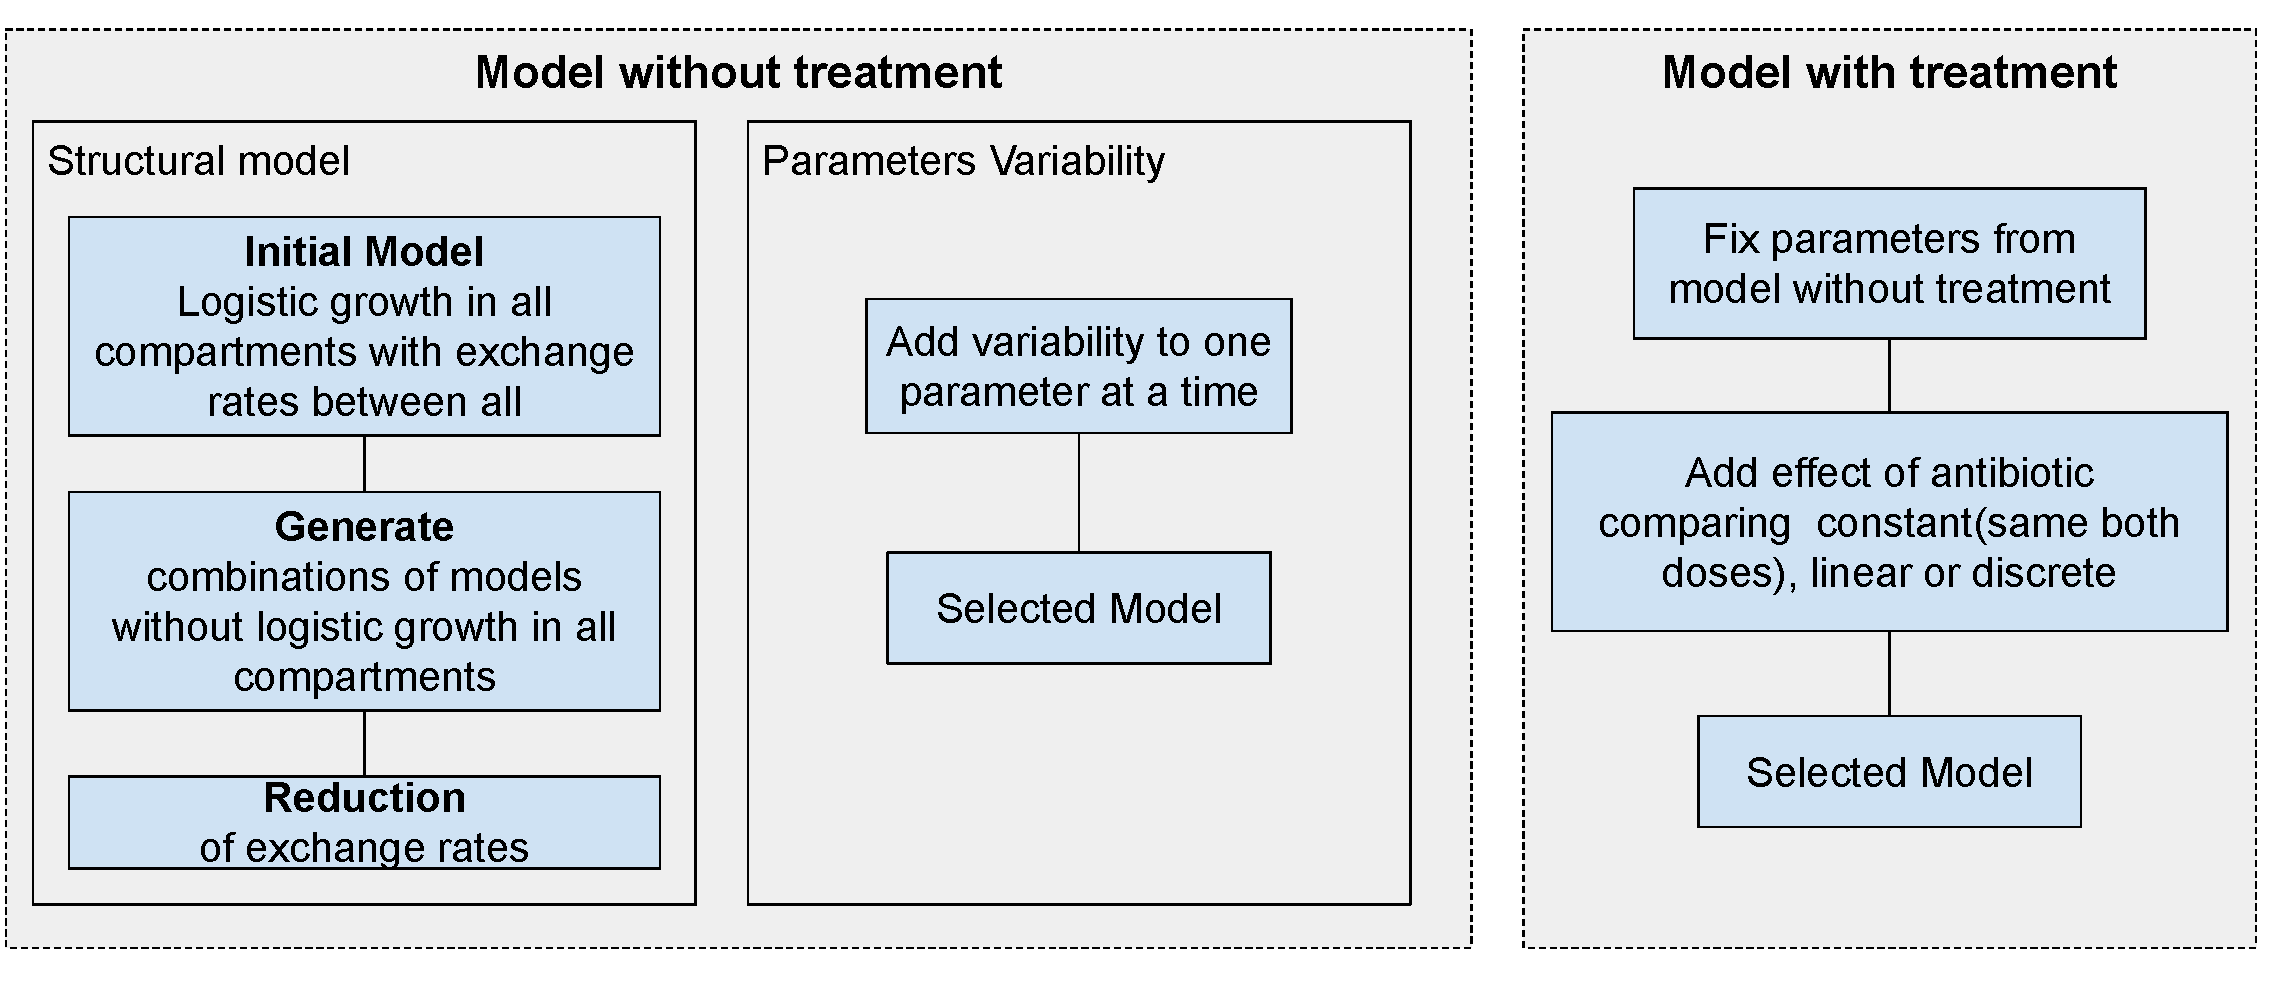
\includegraphics[width=0.8\linewidth]{images/anoruti_model_strategy.pdf}
	\caption{Model diagram for PAS strain without antibiotic treatment. }
	\label{fig:ModelingStrategy}
\end{figure}

\subsubsection{Model without antibiotic treatment in PAS strain}

To investigate the dynamics of bacterial proliferation and migration in a mouse model of urinary tract infection, we examined both a logistic growth model Eq. (\ref{eq:ODElogistic}) and an effective elimination/proliferation rate model Eq. (\ref{eq:ODEeffect}) within a three-compartment framework, representing the kidney($K$), bladder($B$), and urine ($U$). 
%
The model accounted for exchange rates between compartments to capture bacterial migration between compartments.
%
We tested all combinations of logistic growth and effective elimination/proliferation rates across all compartments to comprehensively evaluate their effects on bacterial dynamics.
%
Our initial focus was on the PAS bacterial strain in mice that were not subjected to antibiotic treatment, allowing us to study the natural progression of infection and bacterial spread without external intervention.

\TODO{Should I include the logistic growth equations? I imaging that for completeness I could write it but maybe in the appendix. Or maybe a general equation for one compartment but probably will not be easy to read.}

\begin{figure}
	\centering
	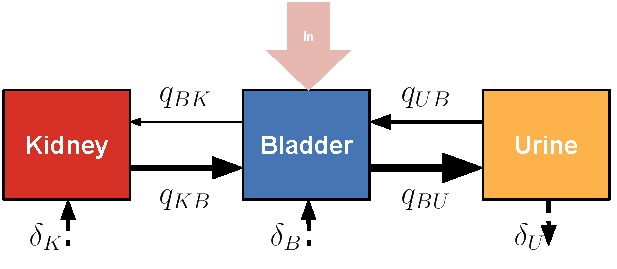
\includegraphics[width=0.8\linewidth]{images/draw_Anoruti_Compartments_oneline_v001.pdf}
	\caption{Model diagram for PAS strain without antibiotic treatment. }
	\label{fig:ModelOnelineNOATB}
\end{figure}

%\begin{alignat}{2}
%\frac{d}{dt} X &=  \alpha_X \left(1 - \frac{X}{X^{ss}} \right) X + \sum_{Y \neq X} \left( - q_{X,Y} X + q_{Y,X} Y \right) & \text{Logistic Growth} \label{eq:ODElogistic} \\
%\frac{d}{dt} X &=  \delta_X X + \sum_{Y \neq X} \left( - q_{X,Y} X + q_{Y,X} Y \right) & \text{Effective elimination/proliferation}
%\label{eq:ODEeffect}
%\end{alignat}



%\begin{equation}
%\frac{d}{dt} X =  \alpha_X \left(1 - \frac{X}{X^{ss}} \right) X + \sum_{Y \neq X} \left( - q_{X,Y} X + q_{Y,X} Y \right)
%\end{equation}


%\begin{equation}
%	\frac{d}{dt} X =  \delta_X X + \sum_{Y \neq X} \left( - q_{X,Y} X + q_{Y,X} Y \right)
%\end{equation}
where $X$ is a compartment $X, Y \in \{K, B , U\}$



\begin{alignat}{2}
\frac{d}{dt} K &=  \alpha_K \left( 1 - \frac{K}{K^{ss}}\right) K &- q_{K,B} K + q_{B,K} B \nonumber \\
\frac{d}{dt} B &=  \alpha_B \left( 1 - \frac{B}{B^{ss}}\right) B &+ q_{K,B} K - q_{B,K} B \nonumber \\
&              &+ q_{U,B} U - q_{B,U} B \nonumber \\
\frac{d}{dt} U &= -\alpha_U \left( 1 - \frac{U}{U^{ss}}\right) U &- q_{U,B} U + q_{B,U} B \label{eq:ODElogistic}
\end{alignat}


\TODO{Net rate of change}
%\begin{equation}
\begin{alignat}{2}
\frac{d}{dt} K &=  \delta_K K &- q_{K,B} K + q_{B,K} B \nonumber \\
\frac{d}{dt} B &=  \delta_B B &+ q_{K,B} K - q_{B,K} B \nonumber \\
&              &+ q_{U,B} U - q_{B,U} B \nonumber \\
\frac{d}{dt} U &= -\delta_U U &- q_{U,B} U + q_{B,U} B \label{eq:ODEeffect}
\end{alignat}
%\end{equation}
where $K$, $B$ and $U$ represents the amount of CFU in kidney, bladder and urine respectively. 
$\delta_K$, $\delta_B$, and $\delta_U$ are effective proliferation rates.  $q_{X,Y}$ the migration rate from compartment $X$ to $Y$ with $X, Y \in \{K,B,U\}$

\subsubsection{Model with antibiotic treatment in PAS strain}

We investigated the effect of the antibiotic ciprofloxacin on mice infected with the PAS strain, focusing on groups that received no treatment as well as those treated with two doses: 2.5 mg/kg and 10 mg/kg. Given the absence of measured drug concentrations, we assumed that the antibiotic primarily influences the effective growth rates of the bacteria. To explore this assumption, we tested three different models: a model with no effect of the antibiotic, a linear model with dose dependence, and a non-linear model to evaluate the impact of the antibiotic on bacterial dynamics.

\begin{alignat}{1}
\delta_{X}^{Cipro} &= \left( 1 \pm \mathcal{A}(D^{Cipro} ) \right) \delta_{X}
\end{alignat}
where $\mathcal{A}(D^{Cipro} )$ is the functional dependency of corresponding administrated dosage, $delta_X$ the effective proliferation rate in the compartment $X \in \{K, B, U\}$.


\begin{alignat}{2}
	\mathcal{A}(D^{Cipro}) &= 0, & \text{No effect} \\
	\mathcal{A}(D^{Cipro}) &= \epsilon_{X} D^{Cipro}, & \text{Linear} \\
	\mathcal{A}(D^{Cipro}) &= \beta_{D^{Cipro}, D_1}\Phi_{D_1} + \beta_{D^{Cipro}, D_2}\Phi_{D_2}, & \text{No linear}
\end{alignat}

\begin{alignat}{1}
\delta_{K}^{Cipro} &= 1 - \epsilon_K D^{Cipro} \delta_{K} \nonumber \\
\delta_{U}^{Cipro} &= 1 + \epsilon_U D^{Cipro} \delta_{U}
\end{alignat}




\subsubsection{Strain covariates}
A forward covariate selection procedure was applied to assess the influence of different bacterial strains on both the elimination/proliferation rates and the exchange rates between compartments. Starting with the PAS strain as the base model, additional bacterial strains were tested individually as covariates. The Bayesian Information Criterion corrected for small sample sizes (BICc) was used to assess model improvement, with strains retained if they led to a reduction in BICc.
%
This process was repeated iteratively, with one covariate added at a time. The final model included only those covariates that significantly reduced BICc.


%\begin{alignat}
%	\frac{d}{dt} X = \alpha_{X} \left( 1 - \frac{X}{X^{ss}} \right)X + \sum_{Y \neq X} q_{X,Y} X + q_{Y,X} Y
%\end{alignat}






%\subsection{Parameter estimation}

\subsection{Model estimation and evaluation}

Estimation of population parameters was performed using the stochastic approximation expectation maximisation algorithm (SAEM) \cite{kuhn2005maximum}, implemented in Monolix 2021R2 (Lixoft, Orsay, France, www.lixoft.eu), a software devoted to parameter estimation by maximum likelihood in nonlinear mixed effect models. Data below the lower limit of quantification were treated as left-censored data. Their contribution to the likelihood was computed as the probability that these data are indeed below the lower limit of quantification\cite{samson2006extension}. 


Model evaluation was carried out using the goodness-of-fit was assessed by inspecting diagnostic plots (e.g., observed vs. predicted values, residuals vs. fitted values)

In addition, model selection was guided by comparing BIC where appropriate. The final model was selected based on the best fit to the data. \TODO{detail model strategy in accordance with new figure 2 to 3.}


\subsection{Simulations}
\TODO{Detail simulations}
\begin{itemize}
	\item Simulations for PAS, and strains, done with simulx, etc
	\item Number of virtual mice?
	\item Definition of time to clearance?
	\item What else could we explore in simulations?
\end{itemize}



\section{Results}

\subsection{Estimated Parameters}

	\begin{table}
	\begin{tabular}{|l|l|l|l|}
		\hline
		Parameter & Estimates(r.s.e.) & Units\\ \hline
		$\delta_{K}$ & $12.2(1.09\%)$ & $(days)^{-1}$\\
		$\delta_{B}$ & $12.7(11.2\%)$ & $(days)^{-1}$\\
		$\delta_{U}$ & $9.75(30.6\%)$ & $(days)^{-1}$\\
		$q_{BK}$ & $0.0021(92.3\%)$ & $(days)^{-1}$\\
		$q_{KB}$ & $12.3(1.06\%)$ & $(days)^{-1}$\\
		$q_{BU}$ & $59.2(35.5\%)$ & $(days)^{-1}$\\
		$q_{UB}$ & $4.24(16.6\%)$ & $(days)^{-1}$\\
		$\omega_{\delta_{U}}$ & $3.36(36.9\%)$ & $(days)^{-1}$\\
		$\omega_{q_{BU}}$ & $0.231(25.3\%)$ & $(days)^{-1}$\\
		\hline
	\end{tabular}
	\caption{Estimates of model without antibiotic treatment, with variabilities in $\delta_U$ and $q_{BU}$ with normal and log-normal distribution respectively.}
\end{table}


\TODO{directly in text, comments with RSE. }
\begin{table}
	\begin{tabular}{|l|l|l|l|}
		\hline
		Parameter & Estimates(r.s.e.) & Units\\ \hline
		$\epsilon_{K}$ & $0.0057(17.4\%)$ & $g/(days.kg)$\\
		$\epsilon_{U}$ & $464.37(30.8\%)$ & $g/(days.kg)$\\
		\hline
	\end{tabular}
	\caption{Parameter estimates for model with antibiotic treatment.}
\end{table}

%final_model_Ct_PAS
\begin{figure}
	\centering
	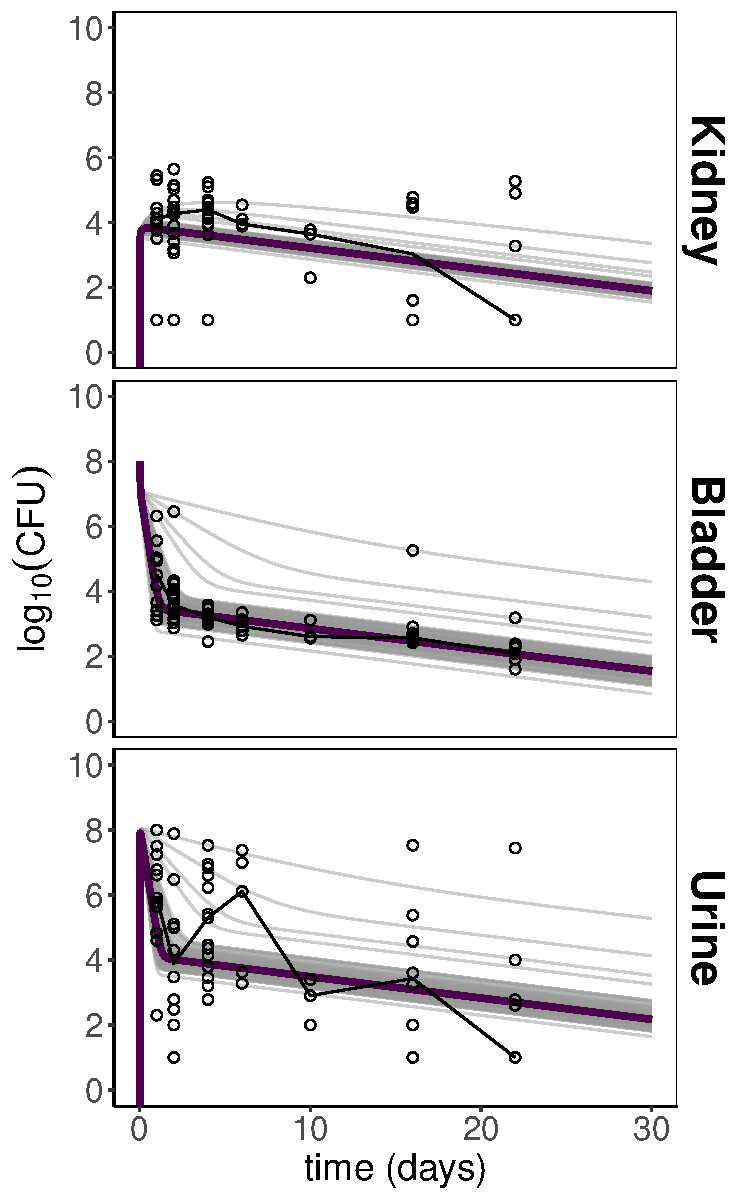
\includegraphics[width=\linewidth]{images/plt_final_model_Ct_PAS_vertical.pdf}
	\caption{Time evolution of CFU for each organ compartment, open circles experimental data, individual fits gray line, purple curve population parameters, black solid line medianvalue at each sampling day}
	\label{fig:ModelIndFits}
\end{figure}

Strain

%plt_Ct_strain_ALL_covar_deltaU.pdf
\begin{figure}
	\centering
	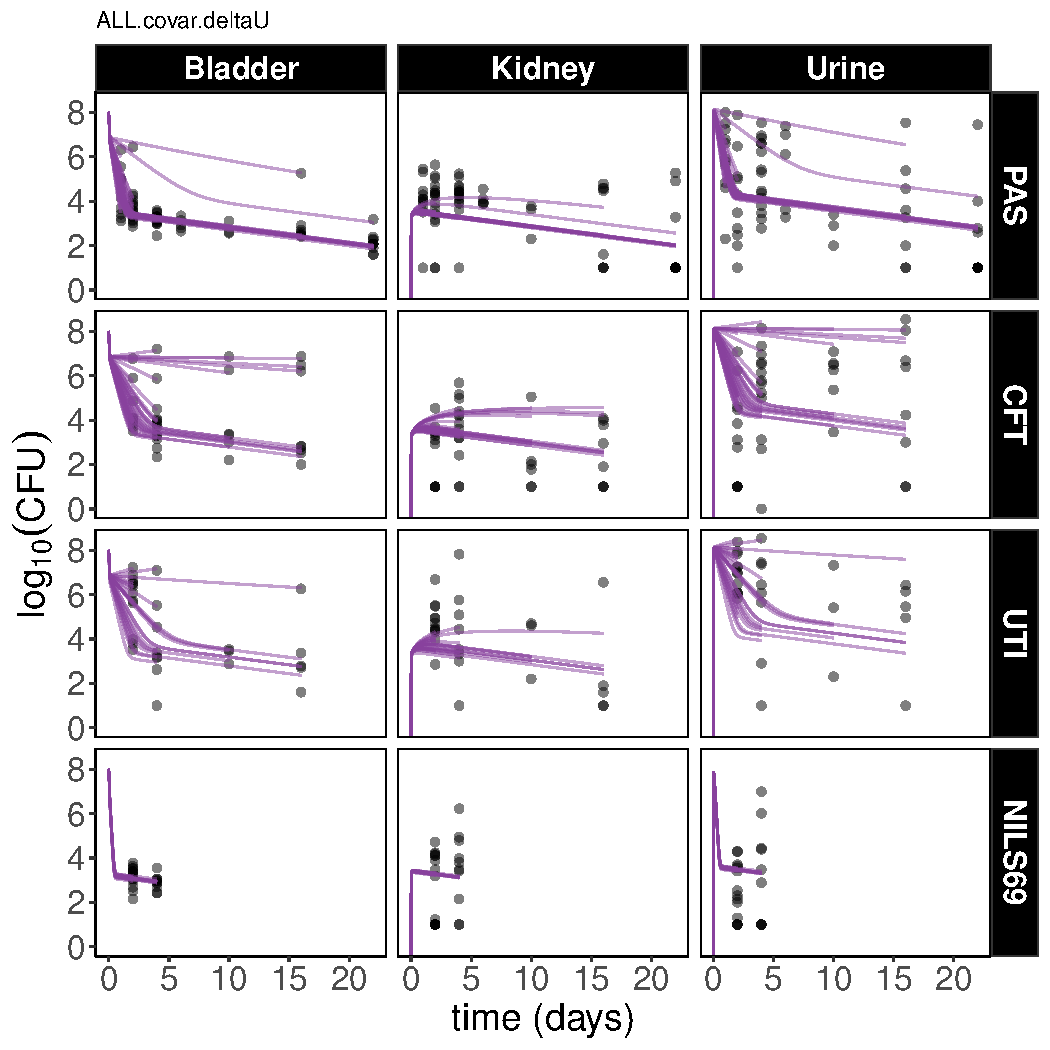
\includegraphics[width=\linewidth]{images/plt_Ct_strain_ALL_covar_deltaU.pdf}
	\caption{Time evolution of CFU for each organ compartment, open circles experimental data, individual fits gray line, purple curve population parameters for different strains.}
%	, black solid line medianvalue at each sampling day
	\label{fig:ModelStrainsIndFits}
\end{figure}



\subsection{Model evaluation}
\TODO{VPC, residuals?}



%plt_vpc_merged_Ct_ONLY.pdf
\begin{figure}
	\centering
	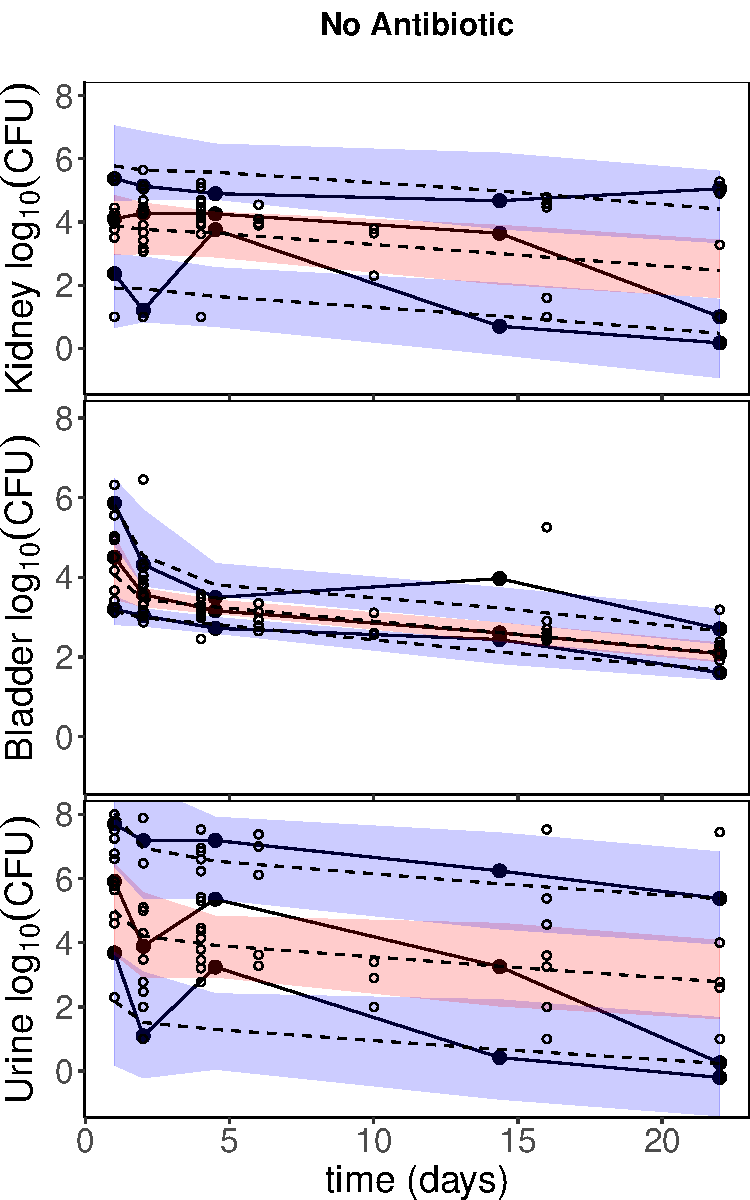
\includegraphics[width=\linewidth]{images/plt_vpc_merged_Ct_ONLY.pdf}
	\caption{Visual Predicte Check for model with antibiotic, for each compartment.}
	\label{fig:ModelIndFits}
\end{figure}


\subsection{Simulations}

\TODO{Add simulations table not only plots}

\section{Conclusions}

\TODO{Fix it}
The competition of bacteria elimination and proliferation are different in the three compartments.
The relationship among bladder, kidney and urine exchange rates indicates that the urine compartment is the main path to elimination and the large proliferation in the kidney positions it as the primary source of a long lasting bacteria. The persistence of bacteria in the bladder despite the administration of ciprofloxacin, even at higher concentrations has been reported before.\cite{jakobsen2020ciprofloxacin} In this study we presented a reduced comprehensive mathematical model of the colonisation in UTI organs for PAS E. coli under the administration of two doses of ciprofloxacin which is the starting point to develop better models with other antibiotics with different mechanism of action and different strains.

Tab. \ref{tab:mice_sampling}

\section{Bibliography}
%\printbibliography %[heading=none,title=none]
\bibliographystyle{plain} % We choose the "plain" reference style
\bibliography{anoruti_refs} % Entries are in the refs.bib file

\appendix
\section{Data}
\TODO{Table Supp.}
\begin{table}[h!]
	\centering
	% Adjust the table size if needed
	\begin{adjustbox}{max width=\textwidth}
%		\begin{tabular}{|c|c|c|c|c|c|c|c|c|c|c|}
		\begin{tabular}{|p{3.5cm}|c|c|c|c|c|c|c|c|c|c|}
			\hline
			\makecell[c]{Antibiotic Group} & \makecell[c]{Strain} & \multicolumn{8}{c|}{Days} & \makecell[c]{Total} \\ \cline{3-10} 
			&                      & 1 & 2 & 4 & 6 & 10 & 14 & 16 & 22 & \\ \hline
			\multirow{4}{*}{Control} & PAS & 13 & 17 & 18 & 5 & 3 &  & 9 & 11 & 76 \\ \cline{2-11}
			& NILS69 &  & 15 & 12 &  &  &  &  &  & 27 \\ \cline{2-11}
			& UTI &  & 12 & 11 &  & 3 &  & 5 &  & 31 \\ \cline{2-11}
			& CFT &  & 11 & 13 &  & 8 &  & 8 &  & 40 \\ \hline
			\multirow{3}{*}{\makecell[c]{Ciprofloxacin 2.5 mg/kg }} % \\ 9 a.m and 5 p.m. \\for 48 hours.
			& PAS &  &  & 17 &  & 5 &  &  &  & 22 \\ \cline{2-11}
			& UTI &  &  & 7 &  &  &  &  &  & 7 \\ \cline{2-11}
			& CFT &  &  & 11 &  &  &  &  &  & 11 \\ \hline
			\multirow{4}{*}{\makecell[c]{Ciprofloxacin 10 mg/kg }} % 9 a.m and 5 p.m. \\for 48 hours.
			& PAS &  &  & 7 &  &  &  &  &  & 7 \\ \cline{2-11}
			& NILS69 &  &  & 7 &  &  &  &  &  & 7 \\ \cline{2-11}
			& UTI &  &  & 7 &  &  &  &  &  & 7 \\ \cline{2-11}
			& CFT &  &  & 6 &  &  &  &  &  & 6 \\ \hline
			\multirow{1}{*}{\makecell[c]{Cefotaxime 100 mg/kg}}  % \\ every 6 hours \\for 24 hours.
			& PAS &  &  & 14 &  & 6 &  &  &  & 20 \\ \hline
			\multirow{1}{*}{\makecell[c]{Fosfomycin 100 mg/kg }} % \\ every 4 hours \\for 24 hours.
			& PAS &  &  & 8 &  &  &  &  &  & 8 \\ \hline
			\multirow{1}{*}{\makecell[c]{Delafloxacin 10 mg/kg }} % \\ 9 a.m and 5 p.m. \\for 48 hours.
			& PAS &  &  & 7 &  &  &  &  &  & 7 \\ \hline
			& & 13 & 55 & 145 & 5 & 14 & 11 & 22 & 11 & 276 \\ \hline
		\end{tabular}
	\end{adjustbox}
	\caption{Mice sampling distribution with antibiotic treatments on bacterial strains in time.}
	\label{tab:mice_sampling}
\end{table}


\end{document}
